\section{The Trading System}
In this section, we present our trading system which uses the trading simulation layer and GA to select and combine trading rules coming both from technical indicators as depicted in the previous section and from our AI layer described in Section~\ref{subsection:ai} to generate buy/sell signals. The trading system uses time series price data of 6 currency pairs: 4 major pairs like GBPUSD, EURUSD, USDCHF and USDJPY, and 2 minor pairs like EURGBP and GBPJPY.

The idea to combine trading rules it is borrowed by the real world of trading, where traders and analysts before opening positions on the market try to confirm their decision suing different approaches and indicators. 

Two phases constitute our proposed trading system: in the first phase, each trading rule, both the AI-based rule and the trading rules from technical indicators, is tested for selection and in the second phase, profitable rules among the qualified rules are selected and combined. Training data is used in the learning step of the trading system.

An overview of the two phases of the proposed framework is illustrated in Fig.~\ref{fig:sys}. In the following sub-sections, the phases of the system are explained in detail.

\begin{figure}[h]
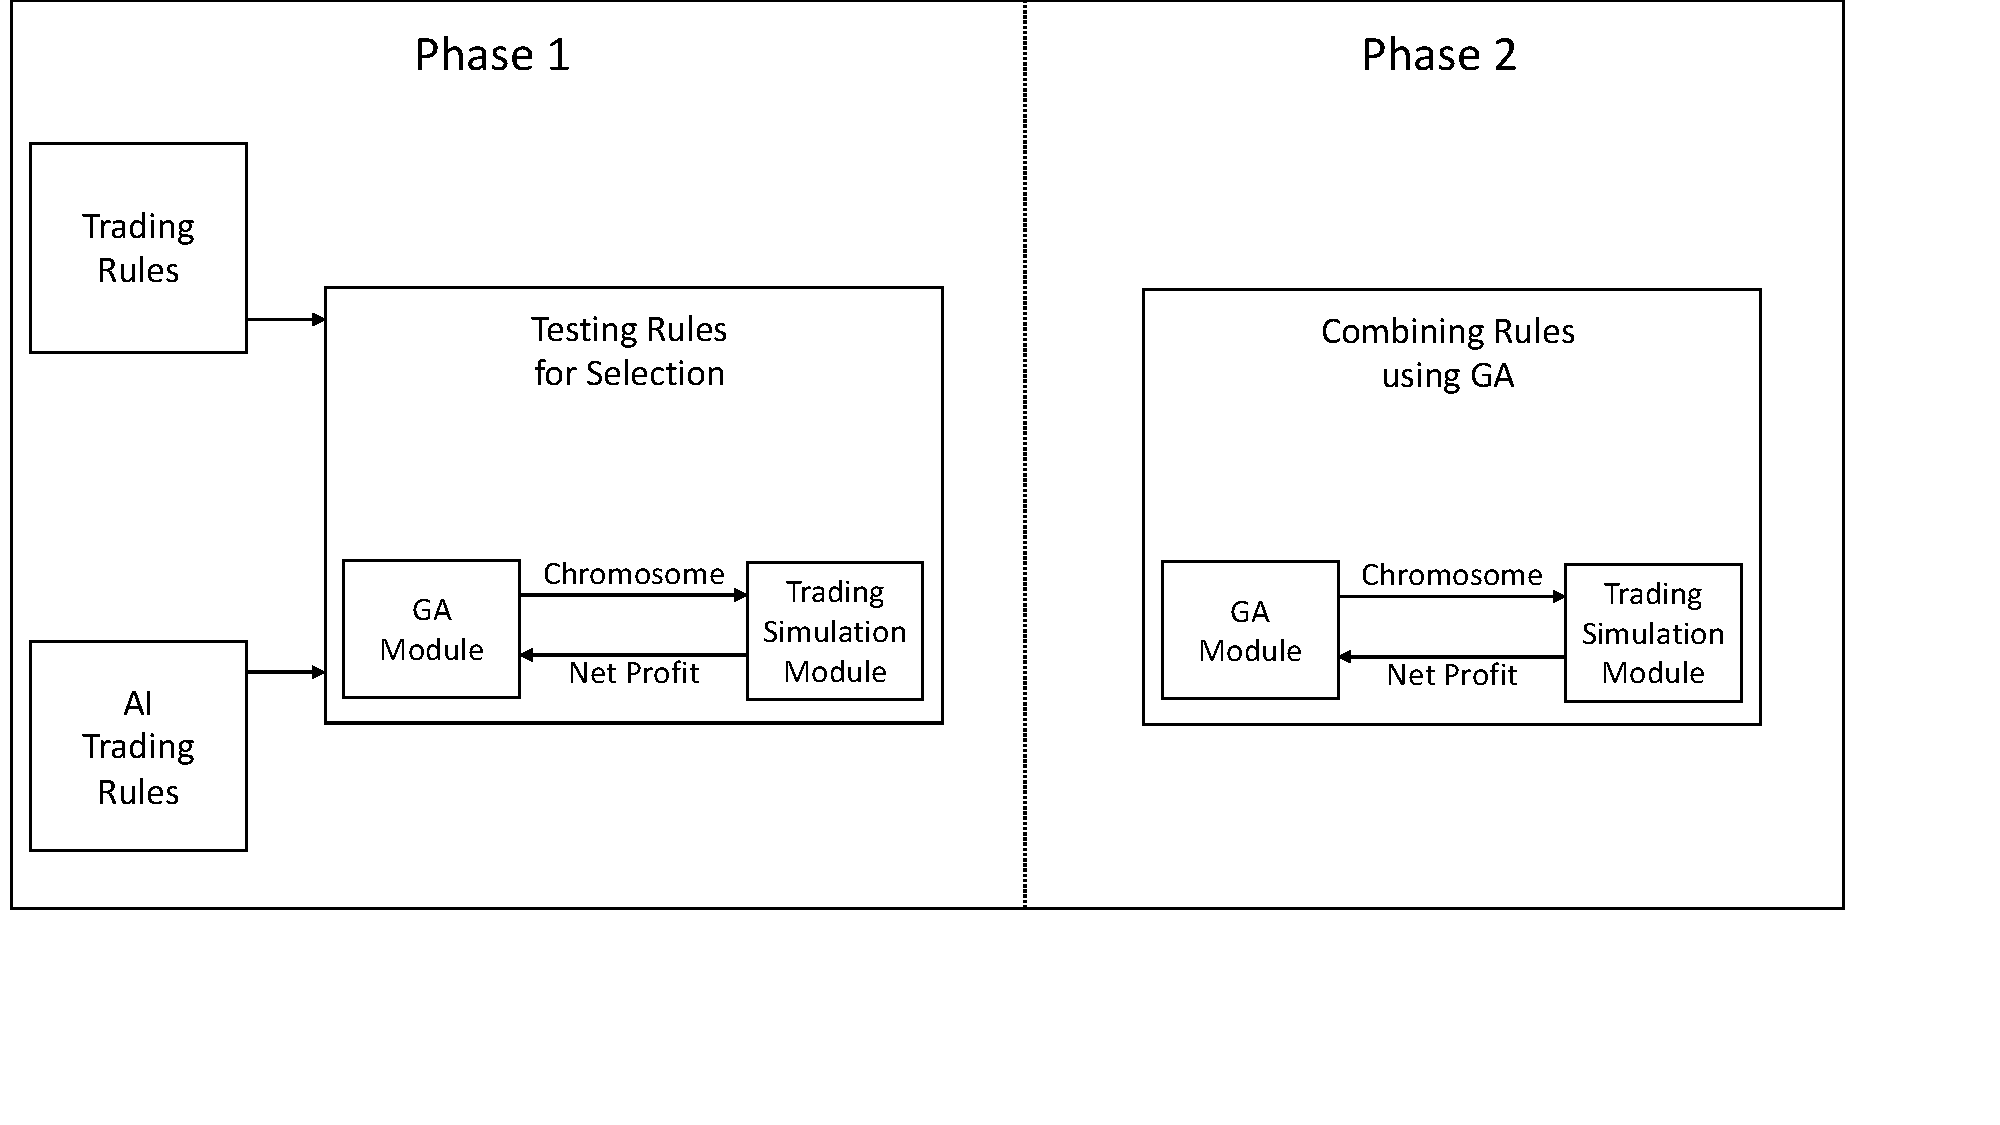
\includegraphics[scale=0.3]{framework}
\centering
\caption{The framework of our trading system.}
\label{fig:sys} 
\end{figure}

\subsection{Phase 1: each trading rule is tested for selection}
The goal of this first phase is the selection of trading rules, both the AI-based rule and the trading rules from technical indicators. Three layers are employed in such a phase: AI (Section~\ref{subsection:ai}), GA (Section~\ref{subsection:ga}) and the Trading Simulation (Section~\ref{subsection:trading})layers. 

As depicted on the left part of Fig.~\ref{fig:sys}, each trading rules from technical indicators discussed in the previous section and for the AI-based rule are given as input to the GA layer which randomly generates chromosomes representing with their genes several parameter combinations both directly related to the specific trading rule (e.g. period $D$ for the Slow Stochastic Oscillator rule) and related to the trade (e.g. the money management risk in percentage, $risk\%$, explained hereafter). Then, all of these candidate rules with several parameter combos are simulated over the historical training data using the Trading Simulation layer which gives as output the Net Profit provided as the fitness value to the GA layer. Following, the best performing chromosome for each rule in term of net profit is selected. 
The rules whose best chromosome does not have a positive net profit are directly eliminated and do not pass to the second phase.


\subsubsection{Trading Simulation Layer}
\label{subsection:trading}
This layer is used to simulate any buying and selling rule on the given time series data with respect to specific currency pairs in order to generate buy/sell/StopLoss/TakeProfit signals (hereafter explained) and calculate net profit as well as different statistics (number trades/deals, total net profit, number of ticks, balance drawdown absolute/max/relative, consecutive wins/profit, consecutive losses, and many others) at the end of the simulation. Our trading simulation system adopts a realistic approach to compute the net profit: we use a demo account with a trading broker \footnote{https://www.icmarkets.com/en/open-trading-account/demo/} simulating the placement of buy/sell positions. Our choice to go through a demo trading account is fundamental for realistically computing the gain and loss of our proposed approach. Finally, the net profit of the simulated trading rule is used as fitness value for the GA layer. 

The simulation of the placement of a buy order is given in Algorithm \ref{alg:tradingSim}. Similarly is done the placement of a sell order.

\vspace{\baselineskip}% Insert a blank line
\SetInd{0.5em}{0.5em}
\begin{algorithm}[H]
\KwIn{

$signal$: A trading signal: trading rule BUY signal to open BUY position; 

$marketMovingHoriz$: Definition of Market moving horizontally; 

$symbol$: The selected currency pair;

$stopLoss$: Initial fixed Stop-Loss in points;

$takeProfitXSL$: Multiplier factor of Take-Profit with respect to Stop-Loss;

$sellPosCount$: The count of open SELL positions;

$fixedVolume$:  Volume in lots;

$riskPercent$:  Maximum risk per trade with respect to the current balance;

}
\KwOut{A list of opened positions}
\While{$OnTick()$}{
$newBar$= CheckNewBar()\;
\If {$(newBar==true)$}{
\tcc{Open BUY position and close all SELL positions}
\If{$(signal==BUY)$}{
\tcc{Close open SELL positions}
\If{$(sellPosCount > 0)$}{
CloseAllSellPosition()\;
}
\tcc{Do not open another BUY if there is a current BUY position opened with a price in a close range}
\If{$(currentBar.Close > (lastPriceBuyOpenPosition + (marketMovingHoriz/2))  ||
currentBar.Close < (lastPriceBuyOpenPosition - (marketMovingHoriz/2))$}
{
\tcc{Compute StopLoss, expressed in points}
$dynamicStopLoss$ = DynamicStopLoss()\;
$stopLossDistance$ = MathMax($dynamicStopLoss, stopLoss$)\; 
\tcc{UseMoneyManagement}
$tradeSize$=MoneyManagement($symbol, fixedVolume, riskPercent, stopLossDistance$)\;
\tcc{takeProfit is X times stopLoss}
$buyProfit$ = BuyTakeProfit($symbol, takeProfitXSL, currentBar.Price$)\; 
\tcc{Buy}
$glBuyPlaced$=TradeBuy($tradeSize, stopLossDistance, buyProfit, symbol$)\; 
}	
}
%\tcc{Open SELL position and close all BUY positions}
%\If{$(signal==SELL)$}{
%\tcc{Close open BUY positions}
%\If{$(buyPosCount > 0)$}{
%CloseAllBuyPosition()\;
%}
%\tcc{Do not open another SELL if there is a current SELL position opened with a price in a close range}
%\If{$(currentBar.Close > (lastPriceSellOpenPosition + (marketMovingHoriz/2)) ||
%currentBar.Close < (lastPriceSellOpenPosition - (marketMovingHoriz/2))$}
%{
%\tcc{Compute StopLoss, expressed in points}
%$dynamicStopLoss$ = DynamicStopLoss()\;
%$stopLossDistance$ = MathMax($dynamicStopLoss, stopLoss$)\; 
%\tcc{UseMoneyManagement. E.g. max Risk can be 10\%of the overall balance}
%$tradeSize$=MoneyManagement($symbol, FixedVolume, RiskPercent, stopLossDistance$)\;
%\tcc{takeProfit is X times stopLoss. If it is zero it is not considered}
%$buyProfit$ = SellTakeProfit($symbol, takeProfitXSL, currentBar.Price$)\; 
%\tcc{Buy}
%$glBuyPlaced$=TradeSell($tradeSize, stopLossDistance, buyProfit, symbol$)\; 
%}	
%}
}
}
\caption{Opening a BUY position}
\label{alg:tradingSim}
\end{algorithm}
\vspace{\baselineskip}% Insert a blank line

We first check if a new bar occurred. This is important to adhere to the respective period chosen, e.g. 1-minute,  5-minute, 15 minutes, an hourly, daily and weekly bar chart and so on.
Secondly, we check if a signal $BUY$ has being triggered. If so, we verify if sell positions are still open and close them. Then, we check if there is another buy position opened previously with a price in a close range of the current one. If so, we do not open a new open position.

\noindent At this point, we compute the trade size using the money management function, the stop loss and the take profit. Finally, we open the buy position. In the following sub sections, the details of the latter computations. 

\paragraph{\textbf{Money Management for computing the trade size}}\mbox{}

Money Management is a procedure to best set position size with respect to risk. Most traders use the same fixed trade volume for every trade. This can result in trades that are too large or too small for the amount of money that is being risked.

To calculate an optimal trade size, we use the distance of the stop loss price from the trade entry price as well as a percentage of the current balance to determine the maximum risk per trade. A good guideline is to limit your risk per trade to 2-4\% of your current balance. This value was computed by our GA layer (more details in Section~\ref{subsection:ga}), where the risk-value is represented as a gene (i.e. $risk\%$) of a chromosome. If for some reason we cannot calculate a trade volume (i.e. stop loss or percentage has not been specified), we will fall back to a specified fixed trade volume.

Let's show the Algorithm~\ref{alg:mm} that explains the $MoneyManagement()$ method of Algorithm \ref{alg:tradingSim}. 

\vspace{\baselineskip}% Insert a blank line
\begin{algorithm}[H]
\KwIn{

$MAXPERCENT$: Is a constant specifying the max risk and set to 10\%

$symbol$: The selected currency pair;

$fixedVolume$:  Default trade volume in lots;

$riskPercent$:  Maximum risk per trade with respect to the current balance;

$stopLossDistance$: Stop Loss distance in points;

}
\KwOut{$tradeSize$: Calculated trade volume}
\eIf {$(riskPercent > 0) \And (stopLossDistance > 0)$}
{
\If {$(riskPercent > MAXPERCENT)$}{ riskPercent = MAXPERCENT\;}
margin = AccountInfoDouble($accountBalance$) * ($riskPercent/100$)\;
tickSize = SymbolInfoDouble($symbol$)\;

tradeSize = ($margin / stopLossDistance$) / $tickSize$\;
tradeSize = VerifyVolume($symbol,tradeSize$)\;

return($tradeSize$)\;
}{
tradeSize = $fixedVolume$\;
tradeSize = VerifyVolume($symbol,tradeSize$)\;
		
return($tradeSize$)\;
}

\caption{Money Management method}
\label{alg:mm}
\end{algorithm}

\vspace{\baselineskip}% Insert a blank line
The $tradeSize$ will hold our calculated trade volume. First we check if $riskPercent$  and $stopLossDistance$ are both greater than zero. If not, then we cannot calculate the trade volume, and we will fall back on the default trade volume specified by $fixedVolume$. Otherwise, if both $riskPercent$  and $stopLossDistance$ are valid, then we will proceed with calculating the trade volume.

Next, we calculate the amount of margin to risk, retrieving the account balance using the AccountInfoDouble() function. Then we retrieve the tick size and store that in $tickSize$. The tick size is the amount of profit or loss represented by a single point move. 

To calculate our trade volume, we divide the margin to risk ($margin$) by the stop loss in points ($stopLossDistance$) and divide the result by $tickSize$. Then we pass our calculated trade volume to VerifyVolume() function. The latter verification is done since most Forex brokers allow trade sizes as small as 0.01 lots, but some brokers have a higher minimum trade size or do not use micro lots.

Let's clarify this with an example. We want to place an order risking no more than $2\%$ of our account balance of \$ $5000$. The initial stop loss will be placed $500$ points away from the order opening price. The symbol is EURUSD and we are using mini lots of $0.1$, so the tick size will be $\$1$ per point. $2\%$ of $\$5000$ is $\$100$, so this value will be saved in the $margin$ variable. The value of the $tickSize$ variable will be $\$1$.
$\$100$ divided by $500$ points is $0.2$. Every point of movement will equakl approximately $\$0.20$ of profit or loss. $0.2$ divided by $\$1$ equals $0.2$, so our trade value will be $0.2$ lots. If this trade of $0.2$ lots hits its initial stop loss $500$ points away, the loss will be approximately $\$100$. If the stop loss distance is $200$ points aways, the trade valume will be $0.5$ lots, but the maximum loss is still $\$100$.

\paragraph{\textbf{Stop Loss and Take Profit}}\mbox{}

Many trading strategies place the stop loss and take profit a fixed distance from the order opening price. The trader specifies the number of points for the stop loss and take profit that are then calculated to the order or position opening price. For a market order, the opening price is the current Bid or Ask price at the moment the order is filled.

\textit{\textit{\textbf{Stop Loss:}}} For a buy order, the stop loss is calculated by subtracting the stop loss value in points from the opening price. For a sell order, the stop loss is calculated by adding the stop loss value in points to the opening price.
First, the symbol's point value is multiplied by the stop loss value. For example, a Forex symbol with five digits after the decimal points will have a point value of $0.00001$. If we have specified a stop loss of $500$ pints, we multiply $500$ by $0.00001$ to get a value of $0.005$. This value is then added or subtracted from the opening price to find the stop loss price.

\textit{\textit{\textbf{Take Profit:}}} As a stop loss price is computed, as well the take profit price is calculated, only in reverse. The take profit price for a buy order is placed above the opening price, while the take profit price for a sell order is placed below the opening price.

One of the most common error made by traders is invalid stop prices. A stop loss or take profit must be a minimum distance away from the current Bid and Ask prices. The minimum distance is called \textit{stop level} and it is retrieved from the broker server. Before we attempt to place an order with our new calculated stop loss or take profit price, we need to verify the price to make sure it is not inside the stop level.

So far we introduced an initial fixed stop loss in points, but there are other ways of determining a stop loss price, such as using an indicator value or a technical support/resistance level. The DynamiyStopLoss() function in Algorithm \ref{alg:tradingSim} retrieves the lowest lowest Low (since we are opening a buy position, otherwise it would have been the highest High) of the last 5 bars and assign the result to $dynymicStopLoss$ variable. For sake of clarity, this value of checking the last 5 bars was computed by our GA layer, where the interval-value is represented as a gene (i.e. $intervalSL$) of a chromosome. The same was, we computed the gene $takeProfitXSL$, as the multiplier factor of take profit with respect to stop loss, in points, and found out the best value equal to 2.

We conclude this paragraph introducing the trailing stop. A trailing stop is a stop loss that moves as a position increases in profit. For a buy order, the trailing stop moves up in price as the position gains in profit, and for a sell order, the trailing stop moves down in price as the position gains in profit. A trailing stop typically follows the current price by a specified number of points, defined in our algorithm as $trailingStop$ variable. For example, if a trailing stop is set to $500$ points, then the stop loss begins moving once the current price is at least $500$ points away from the stop loss price. We can delay a trailing stop by requiring a minimum level of profit be reached first, specified in our algorithm as $minProfit$ variable. Both $trailingStop$ and $minProfit$ values are computed by our GA layer as values of genes of a chromosome; the best output was found with $trailingStop$ equal to $450$ points and $minProfit$ equal to $700$ points. 

Until now, we presented a fixed trailing stop, but we trailed also dynamically following an indicator, such as the Parabolic Stop and reverse (PSAR) indicator. The PSAR was used to set as stop loss that progressively moves closer to the high or low of the current bar. When the PSAR value gets close, or the trend reverses, the PSAR will reverse direction. If the PSAR is below the current bar, then we trail the stop for an open buy position. If the PSAR price is above the most current bar, then we will trail the stop for an open sell position. In our system, the usage or not of the dynamic trailing with PSAR indicator was evaluated by the GA layer of Phase 2 using a binary gene in the chromosome, which discarded its usage.

\paragraph{\textbf{Computing the total net profit}}\mbox{}

The last step of trading simulation layer is the computation of the total net profit.  
For each open position that is closed, either due to reverse signal triggered by our system or meeting the stop loss or meeting the take profit, a profit or loss is computed. The sum of all the gains/losses in the entire temporal window under consideration for a specific currency pair constitutes our total net profit.


\subsubsection{AI Convolutional Layer}
\label{subsection:ai}


\subsubsection{The GA layer: a Genetic Algorithm for variables' parameters selection}
\label{subsection:ga}
The unstable and chaotic structure of exchanges in FX market complicates forecast analysis. This leads to the utilization of optimisation methods. There are many heuristic methods, such as genetic algorithm (GA), simulated annealing (SA), etc. to resolve optimisation problems. Heuristic algorithms are extensively used for solving problems of high computational complexity, alternatively of going via all of the options, which takes up a considerable quantity of time. GA is one of the most popular heuristic optimisation approach that generates options which evolve in time \cite{OZTURK2016170}. GA is based totally on evolution and genetics. Heuristic strategies yield nearly but not necessarily optimal solution with reasonable computational effort and time.

Genetic algorithm refers to the heuristic algorithm, which offers an acceptable answer to the hassle in the majority of virtually practically significant cases, however the correctness of the decisions has no longer been tested mathematically, and is used most frequently for problems, the analytical solution of which is very hard or even impossible.

GA contains the concepts, borrowed from nature. These are the ideas of heredity and variability. Heredity is the capacity of organisms to transmit their traits and evolutionary characteristics to their offspring. Thanks to this capability, all living organisms pass the characteristics of their species in their offspring.

The variety of genes in living beings assures the genetic variety of the population and is random, considering nature would not have a manner of knowing in advance which characteristics may be most useful for the future (weather exchange, famine, dryness and so forth.). This variability allows the appearance of creatures with new features, which could live in the new environmental conditions and transmit the new traits to the offspring.

In GA there are two types of variations carried out within the algorithm: (i) the mutation, which is the variability arising due to the emergence of mutations; (ii) combination which arises from the aggregate of genes with the aid of mating.

The \textit{gene} is the basic unit of information transfer: a structural and functional unit of heredity, which controls the development of a particular features or trait. We are able to call one variable of the function the gene. The gene is represented via a actual quantity: a real number. The set of gene- variables of the studied characteristic is the characterizing characteristic of the \textit{chromosome}.

The chromosome representation of the  Slow Stochastic Oscillator rule is illustrated in Table \ref{tab:Chromosome} as an example, where the period $K$, the period $D$ and $Slowing$ are the genes directly related to the oscillator, while the genes representing the interval of the stop loss, $intervalSL$, the multiplier factor of take profit with respect to stop loss, $takeProfitXSL$, the money management risk in percentage, $risk\%$, the trailing of the current price by a specified number of points, $trailingStop$, and the minimum profit for activating the trailing stop, $minProfit$, are the genes related to the trade.

\begin{center}
\begin{table}[htb]
\centering
\begin{tabular}{|c|c|c|c|c|c|c|c|}
\hline 
K & D & Slowing & intervalSL & takeProfitXSL & risk\% & trailingStop & minProfit\\ 
\hline 
10 & 3 & 6 & 5 & 2 & 2 & 500 & 700\\ 
\hline 
\end{tabular} 
\caption{\label{tab:Chromosome}Chromosome representation of the  Slow Stochastic Oscillator rule.}
\end{table}
\end{center}

All samples of the identical evolutionary era are mixed into a population. Furthermore, the population is arbitrarily divided into two identical colonies: the parent and the descendant colonies. Due to crossing the parental species, which are decided on from the whole population, and different operators of the GA, there is a colony of offspring, which is identical to half the scale of the population.

In our work, the GA algorithm layer is implemented within the MetaTrader 5 platform~\footnote{https://www.metatrader5.com/en/trading-platform}.
Hereafter we report the steps on how the GA layer works:

\begin{enumerate}
\setlength\itemsep{0.3em}
\item Firstly, a range of values as function of start-stop-step values is defined for each gene of a chromosome.
\item Secondly, the chromosomes which represent the parameter combos are randomly generated to shape an initial proto-population.
\item Thirdly, for each chromosome the fitness value is computed and sent to be simulated into the Trading Layer.
\item Finally, we run the main loop of the GA until the selected number of offspring iterations are generated:
\begin{itemize}	
	\item Making ready the population for reproduction, after disposing of chromosome duplicates.
	\item Isolation and protection of the reference chromosome (with the best fitness cost).
	\item For each mating and mutation, new parents are picked up on every time, getting ready the population for the subsequent era.
	\item Evaluation of genes of the best offspring with the genes of the reference chromosome. If the chromosome of the best offspring is higher than the reference chromosome, then replace the reference chromosome.
\end{itemize}
\end{enumerate}

We experimented with several parameters' values in order to tune the GA. For sake of clarity, there are no universal parameters' values, and it is a good practice to assign them on the basis of the domain. We varied the scale of the population, which range between 64 and 256, and the threshold value of the epochs number. We did not choose too large values, since this did not accelerate finding solution to the problem. 
As a result, we have observed the subsequent parameter settings for GA pretty exceptional for our problem (Table~\ref{tab:GAPS}):

\begin{table}[htb]
\centering
\begin{tabular}{|c|c|c|}
\hline 
\textbf{Number of chromosomes in the colony} & 100 \\ 
\hline 
\textbf{Number of epochs without progress} &  50\\ 
\hline 
\textbf{Probability of mutation of each gene in \%} &  5\\  
\hline 
\end{tabular} 
\caption{\label{tab:GAPS}GA parameter settings.}
\end{table}


The following optimization criteria were considered for GA and used with the fitness metric:
\begin{itemize}
\setlength\itemsep{0.3em}
\item Balance max - the highest value of the balance.
\item Net Profit max - the highest value of the net profit.
\item Expected Payoff max - a statistically calculated value showing the average return of one deal.
\item Drawdown max - difference between the initial deposit and the minimal level below initial deposit throughout the whole testing period.
\item Recovery Factor max — the highest value of the riskiness of the strategy, i.e. the amount of money risked by the Expert Advisor to make the profit it obtained.
\item Sharpe Ratio max — the highest value of the efficiency and stability of a strategy. It reflects the ratio of the arithmetical mean profit for the position holding time to the standard deviation from it.
\end{itemize}

For our GA layer, we decided to use as fitness metric the net profit.
In conclusion, the output of the GA layer is a chromosome which has the greatest fitness value discovered.
%https://www.mql5.com/en/articles/55

\subsection{Phase 2: selecting and combining profitable rules}
From the first phase we get for each trading rule, both from technical indicators and AI-based, the best chromosome which has the best fitness value. The rules whose best chromosome does not have a positive net profit are directly eliminated and do not pass to this second phase, where the qualified rules are combined to form a trading system. Two layers are used for the selection of the combo trading rules: GA layer and again the Trading Simulation layer, as employed in the first phase.

As depicted on the right part of Fig.~\ref{fig:sys},